\chapter{Introduction}

A geographic information system (GIS) is a computer system used to capture, store, query, analyze, and display geospatial data. \textbf{Geospatial data} describes both the location and the characteristics of spatial features: for example, if we want to describe a road, we may refer to its location and its features (length, name, speed limit, etc.). Other than single entities, geospatial data can also describe trajectories, specifying the sequence of locations constituting it.\\
The following chapter will give an overview of the basic concepts used in GISs and spatial data analysis.

\section{Geographic Coordinate Systems}

When using a GIS, any map layers used together must align spatially; to make sure this is true, we need to use some common spatial reference system for all maps. GIS users normally work with locations expressed on a plane using a coordinate system expressed in x- and y-coordinates, while the actual, real-life locations represented by them are on Earth's surface (which is ellipsoidal). A \textbf{map projection} is used to convert the Earth's surface to a plane.

The system used to locate points on Earth is called \textbf{geographic coordinate system}. This system is defined by two coordinates: \textbf{longitude} and \textbf{latitude}. They are angular measures which measure the angle at which the point can be found with respect to the \textbf{prime meridian} and the \textbf{equator}; longitute represents the angle east or west from the prime meridian, while latitude represents the angle north or south of the equatorial plane.

\textbf{Meridians} are lines of equal longitude. The prime meridian passes through Greenwich, England, and corresponds to 0°. \textbf{Parallels} are lines of equal latitude. The equator is the line corresponding to 0° latitude.

In a \textbf{plane coordinates} system, longitute and latitude correspond to x and y coordinates respectively. Logitude takes positive values in the easter hemisphere, and negative values in the western hemisphere; latitude takes positive values north of the equator, and negative values south of the equator.
\\
Longitute and latitude values may be expressed in different ways:
\begin{itemize}
    \item \textbf{Decimal degrees} (\textbf{DD}): represented by a single decimal value;
    \item \textbf{Degrees-minutes-seconds} (\textbf{DMS}): represented by a set of three values, corresponding to degrees, minutes, and seconds. 1 degree corresponds to 60 minutes, and 1 minute corresponds to 60 seconds;
    \item \textbf{Radians} (\textbf{rad}): similar to DD, but expressed in radians instead of decimal values: 1 degree is equal to 0.01745 rad.
\end{itemize}

As mentioned before, planet Earth can be approximated as an \textbf{ellipsoid}: this shape is obtained by rotating an ellipse by its shortest axis. Indeed, Earth is wider along the equator (its major axis) than it is between the poles (its minor axis). Another parameter that describes an ellipsoid is the \textbf{flattening} ($f$), calculated as $f = \frac{maj - min}{maj}$, and it describes the difference between the two axes.

A \textbf{datum} is a mathematical model of the Earth which is used as the reference to calculate the geographic coordinates of a point (or even the elevation, if we consider vertical datums). A datum is defined as: the pair \textit{longitude, latitude} of coordinates of an initial point wich will be the origin, an ellipsoid, and the separation of the ellipsiod and the Earth at the origin.

Distances on the Earth's surface are not straight lines; they are instead represented by \textbf{geodesics}: through any two points (not antipodal), there is exactly one ``great circle'' that connects them. The two points separate the great circle in two parts: the shorter of the two is their geodesic distance. Since the Earth is nearly spherical, geodesic distances are correct with an error up to $0.5\%$. The geodesic distance between points $A$ and $B$ is calculated as:
\begin{equation*}
    \cos(d) = \sin(\textit{lat}_A) \sin(\textit{lat}_B) + \cos(\textit{lat}_B) + cos(\textit{lon}_A - \textit{lon}_B),
\end{equation*}
where $d$ is the angular distance between the two points.

\section{Trajectories, Tessellations, Flows}

Let $u$ be an individual. A \textbf{trajectory} $T_u = \langle p_1, p_2, \dots, p_{nu} \rangle$ is a time-ordered sequence composed by the spatio-temporal points visited by $u$. A spatio-temporal \textbf{point} is a pair $p = (t,l)$, where $t$ is the time, and $l=(x,y)$ is the point visited at that time.

Given an area $A$, a \textbf{tessellation} is a set of geographical polygons with the following properties:
\begin{itemize}
    \item It contains a finite number of polygons called \textbf{tiles}:
    \begin{equation*}
        \mathbb{G} = \{g_i : i = 1, \dots, n\}
    \end{equation*}
    \item The tiles are non overlapping:
    \begin{equation*}
        g_i \cap g_j = \emptyset \,, \forall i \neq j
    \end{equation*}
    \item The union of all tiles completely covers the tessellation:
    \begin{equation*}
        \bigcup_{i=1}^n g_i = A
    \end{equation*}
\end{itemize}
A tessellation can be \textbf{regular} or \textbf{irregular} depending on the shape of its tiles. Regular tessellation may use equilateral triangles, squares, hexagons; irregular tessellation may use buildings, census cells, administrative units. A \textbf{spatial join} is used to associate a point with the tile it belongs to. Since the tiles are non overlapping and cover the entire area, each point belongs to one and only one tile. \textbf{Voronoi tesselations} are a particular type of tessellation that partition the plane into regions (called \textbf{cells}), each closer to a secific point (called \textbf{seed}) out of a set. Each of these cells is defined as the set of points that are closest to the seed of the cell itself than any other seed in that area.

Given a tessellation, the \textbf{flow}
\begin{equation*}
    y(g_i. g_j)
\end{equation*}
represents the number of people/objects moving between $g_i$ and $g_j$. A trajectory refers to a single entity, while a flow refers to the total amount of entities moving between two points. Flows can be derived from a set of trajectories, but the inverse is not true.

\section{Raster and Vector Data Models}

The raster and vector data models are two ways to represent geographic information in GISs. In both cases, data can be stored in several \textbf{thematic layers}, each of which contains a set of objects of the same nature. For example, a layer may contain information about buildings, another about streets, another about rivers, and so on.

The \textbf{raster data} model divides the space into a regular grid of square cells with a given size (which defines the \textbf{resolution}). This format is often used for images, where each element corresponds to a pixel. Depending on how much information is assigned to a cell, data can be \textbf{single-band} (one attribute per cell), or \textbf{multi-band} (several attributes per cell). Raster data is typically sourced from satellites.

The \textbf{vector data} model uses discrete objects (points, lines, polygons) to represent spatial features. Each object can have its own properties and relationship with the others. A \textbf{point} is a zero-dimensional object with a \textit{location} property (expressed as x,y coordinates). A \textbf{line} in a one-dimensional object with two properties: \textit{location} and \textit{lenght}. It be either straight or curved. A \textbf{polygon} is a two-dimensional object with three properties: \textit{location}, \textit{area}, and \textit{perimeter}. These objects are expressed differently depending on the data format used by the software/platform.

Objects in a layer are sometimes also called \textit{spatial features}; for this reasin, the variables associated to them are called \textit{attributes} (and not features). To represent geometric objects in a GIS, we can use one of the following models:
\begin{itemize}
    \item \textbf{Geo-relational data model}, where objects and attributes are stored separately, and associating each object to the corresponding attributes requires a join operation (at the advantage of possibly saving space if a certain attribute(s) is (are) only possessed by few objects);
    \item \textbf{Object-relational data model}, where objects and attributes are stored together in a single table, making retrieval much faster (but possibly increasing the amount of space needed to store everything). 
\end{itemize}

In principle, vectors can model everything; raster data is a discretized view of the same information. Raster data is better suited for ``dense'' data; it can be more efficient in those cases where a raster representation may need a very high number of objects, but precision is not a concern. Vector data can also be converted to raster data, and vice versa. \textbf{Rasterization} is the process of transforming vector data into raster data, and produces a discrete approximation. \textbf{Vectorization} is the inverse process: it may be difficult at times, and many algorithms and methods have been developed to perform it.

At times, vectors and raster information can be used together in multi-layer data. Some information is better modeled with one format than the other: for example, street networks or locations of interest are often encoded as vector layers, while things like land usage are encoded as raster layers.

\section{Spatial Operations}

The most important spatial operations are:
\begin{itemize}
    \item \textbf{Intersection}: returns all the points in common with the operands.
    \item \textbf{Union}: returns the union of the two operands. In some tools, They are kept as separate objects, meaning that the result is always a multipolygon. As an alternate operation, the same tools offer the \textbf{dissolve} operation, which instead merges the two objects into a single one.
    \item \textbf{Difference}: returns all the points in the first operand which are not in the second.
    \item \textbf{Buffering}: creates a buffer, i.e., an expanded area, around the object. The result is equivalent to replacing each point in the geometry with a circle with a given radius.
    \item \textbf{Spatial join}: like in relational databases, joins merge the information of two objects. THe join can be \textbf{inner} (the output contains only pairs in common with both objects), or \textbf{outer/left/right} (the output also contains non matching objects with the \textit{NULL} value in place of the missing attributes). 
\end{itemize}

\section{Spatial Patterns and Spatial Correlation}

\textbf{Point Pattern Analysi}s (\textbf{PAA}) is the study of point patterns, i.e., the spatial distribution of points in an area. Spatial distributions are typically categorized into three types:
\begin{itemize}
    \item \textbf{Uniform (discrete)}: points are evenly distributed in the area;
    \item \textbf{Random}: points are distributed according to a random process;
    \item \textbf{Clustered}: points appear to be grouped (clustered) in some areas.
\end{itemize}
A basic form of point pattern analysis consists in determining summary statistics such as mean center, standard distance, and standard deviational ellipse. \\
\textbf{Mean center} is the average of the x and y coordinate values:
\begin{equation*}
    \bar{s} = \left( \frac{\sum_{i=1}^n x_i}{n} , \frac{\sum_{i=1}^n y_i}{n} \right)
\end{equation*}
\textbf{Standard distance} measures the variance between the average distance of the features to the mean center:
\begin{equation*}
    d = \sqrt{\frac{\sum_{i=1}^n (x_i - \mu_x)^2 + (y_i - \mu_y)^2}{n}}
\end{equation*}
Similar to standand distance, \textbf{standard deviational ellipse} measures the standard distances for each axis:
\begin{align*}
    &d_x = \sqrt{\frac{\sum_{i=1}^n (x_i - \mu_x)^2}{n}} \\
    &d_y = \sqrt{\frac{\sum_{i=1}^n (y_i - \mu_y)^2}{n}}
\end{align*}

\textbf{Average Nearest Neighbor} (\textbf{ANN}) is an algorithm that can be used to study patterns. For each point, its nearest neighbor is found as the point with the smallest distance to it. The average of all points' nearest neighbor distance is calculated as $d_{obs}$, and normalized with regards to the expected average if the pattern were random ($d_{exp}$), obtaining a ratio:
\begin{equation*}
    R = \frac{d_{obs}}{d_{exp}}
\end{equation*}
If $R = 1$, the pattern is random. If $R < 1$, the pattern is clustered, because the distances are smaller than expected; if $R > 1$, the pattern is uniform (or at least more dispersed than random).

\textbf{Ripley's K-function} is another popular method for analyzing point patterns. Usually, its normalized version, called \textbf{L function}, is used. Given $n$ points in an area of size $A$, and a distance $d$, the L function is calculated as follows:
\begin{enumerate}
    \item Compute all $n*(n-1)$ distances between each pair of points;
    \item Compute $\phi$, the fraction of distances that are $ \leq d$;
    \item Compute
    \begin{equation*}
        L(d) = \sqrt{\frac{A}{\pi} \phi} \,.
    \end{equation*}
\end{enumerate}
$L(d) = d$ for random distributions. If $L(d)$ is higher, the data is more clustered; if it is lower, the data is more dispersed. Different values of $d$ can be explored to understand patterns at different spatial granularities.

Another important aspect is \textbf{density based analysis}. Density measurements can be either global or local. \textbf{Global density} is simply calculated as the ratio of observed points and the study region's area:
\begin{equation*}
    \hat{\lambda} = \frac{n}{A}
\end{equation*}
Density can also be measured at different locations of the study region. \textbf{Local density} is computed over a single tessellation cell; the chosen resolution will affect the resulting density calculation. \textbf{Kernel density} is another method of calculating density per-cell which considers also the points found in its neighborhood. Usually, given a cell $c$, the 8 adjacent cells are considered as the neighborhood $N_c$, and so the kernel density becomes:
\begin{equation*}
    \textit{Kernel density} \ (c) = \hat{\lambda}(c \cup N_c)
\end{equation*}
A variant is \textbf{weighted kernel density}, which assigns to each point a weight inversely proportional to the distance from the cell's center. Different weight functions can be used; a common one is the Gaussian function.

Autocorrelation is the correlation of the values of a same variable measured at different points in time (\textbf{temporal autocorrelation})/space (\textbf{spatial autocorrelation}). An example of spatial autocorralation may be checking how much the temperature values in the points of a layer are influenced by the neighboring values. According to \href{https://en.wikipedia.org/wiki/Tobler%27s_first_law_of_geography}{\textbf{Tobler's first law of geography}}, ``everything is related to everything else, but near things are more related than distant things'': this is the fundamental assumption in spatial analysis.

Popular measures of spatial autocorrelation are:    
\begin{itemize}
    \item \textbf{Moran's I}, which calculates the autocorrelation between values of each point against all other points in its neighborhood:
    \begin{equation*}
        I = \frac{\sum_{i=1}^n \sum_{j: x_j \in N_{x_i}} w_{ij} (x_i - \mu_x)(x_j - \mu_x)}{s^2 \sum_{i=1}^n \sum_{j: x_j \in N_{x_i}} w_{ij}} 
    \end{equation*}
    where $s^2$ is the variance of the $x$ values, and $w_{ij}$ is a weight, typically defined as the inverse of the distance between the two points. Positive values mean positive correlation, negative values mean negative correlation;
    \item \textbf{Geary's C}:
    \begin{equation*}
        C = \frac{n-1 \sum_{i=1}^n \sum_{j: x_j \in N_{x_i}} w_{ij} (x_i - x_j)^2}{2 (\sum_{i=1}^n \sum_{j: x_j \in N_{x_i}} w_{ij}) * \sum_{i=1}^n (x_i - \mu_x)^2}
    \end{equation*}
    The higher it is, the more different are nearby values (less correlation), the lower it is the closer they are (more correlation).
\end{itemize}
Both measures can also be interpreted as the average of local I/C values calculated across neighborhoods. These local values can be studied individually as well.

\section{Spatial Interpolation}

Spatial interpolation refers to the process of using points with known values (called \textbf{control points}) to estimate values at others. For example, we could estimate the temperature at a point with no recorded data by approximating it from known temperatures at nearby points. Ideally, control points should be well distributed across the study area, although this situation is rare in real-world applications since a study area oftentimes also contains data-poor areas.

Interpolation methods can be divided in two groups: \textbf{deterministic} and \textbf{stochastic}. The first group assumes that the known values are exact, with no assessment of errors for predicted values. The second group considers the presence of some random error in the known data and offers some assessment of prediction error with an estimated variance.
\begin{figure}[!ht]
    \centering
    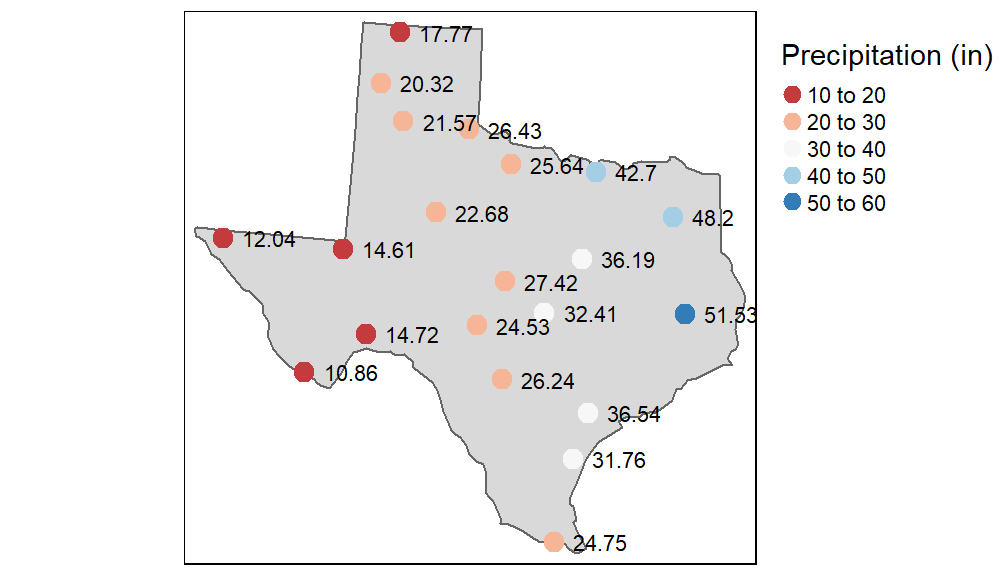
\includegraphics[width=0.5\textwidth]{img/interpolation_original.png}
    \caption{An example of samples corresponding to yearly precipitation recorded in different sites in Texas.}
    \label{fig:interpolation_original}
\end{figure}

\subsection{Deterministic Methods}

\subsubsection{Proximity Interpolation}

Proximity interpolation (also known as \textbf{Thiessen interpolation}) is one of the simplest and oldest interpolation methods. The goal is to assign to all unsampled locations the value of the closest sampled location, producing a Voronoi tessellation over the study area. All the points within the same cell have the same value. A problem of this approach is that surface values change abruptly across the perimeter of adjacent cells, which is not realistic.

\subsubsection{Inverse Distance Weighted Interpolation}

Inverse Distance Weighted (IDW) interpolation calculates an average value using nearby weighted locations. The weight of each sample location is inversely proportional to the distance; the value at location $j$ is given by:
\begin{equation*}
    \hat{Z}_j = \frac{\sum_i Z_i / d_{ij}^n}{\sum_i 1 / d_{ij}^n}
\end{equation*}
Here, $d_{ij}$ is the distance between points $i$ and $j$, and $n$ is an hyperparameter that controls the irrelevance of a point as the distance increases/decreases: the larger $n$ is, the less far away samples influence the interpolated value. For $n \rightarrow \infty$, the result is equivalent to proximity interpolation. \\
Values returned by this method are always within the range of the known values: $[Z_{min}, Z_{max}]$.

\begin{figure}[ht!]
    \centering
    \begin{minipage}{0.49\textwidth}
        \centering
        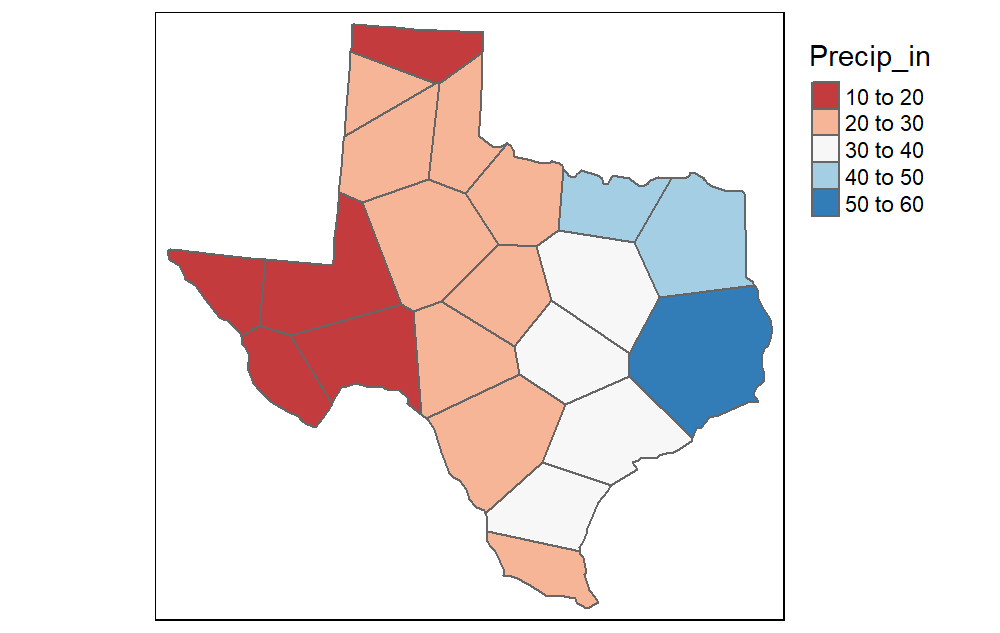
\includegraphics[width=\textwidth]{img/interpolation_proximity.png}
        \caption{Interpolated values obtained by proximity interpolation.}
        \label{fig:interpolation_proximity}
    \end{minipage}
    \hfill
    \begin{minipage}{0.49\textwidth}
        \centering
        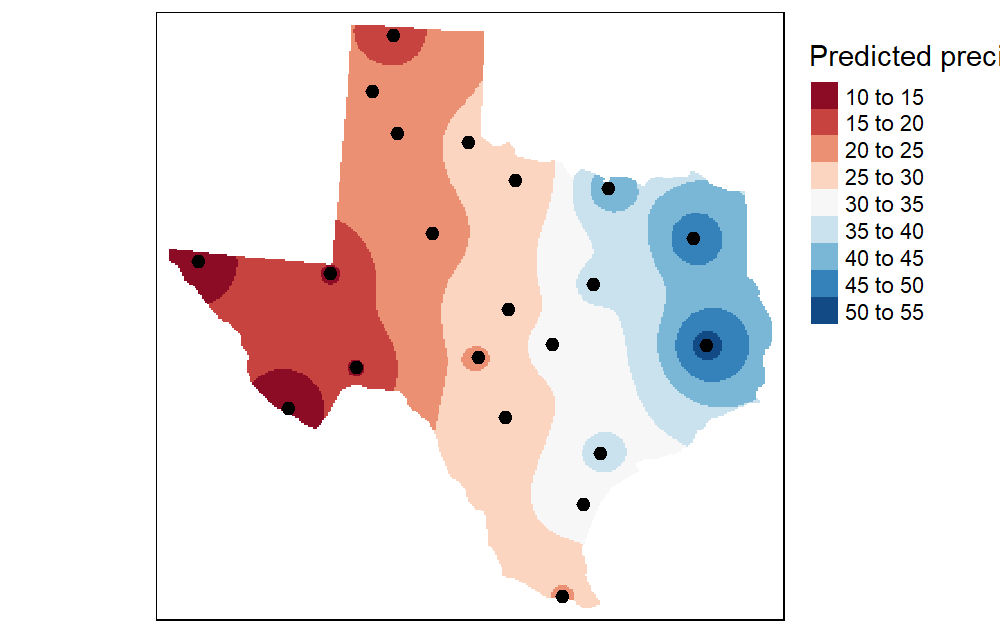
\includegraphics[width=\textwidth]{img/interpolation_idw.png}
        \caption{Interpolated values obtained by IDW interpolation.}
        \label{fig:interpolation_idw}
    \end{minipage}
\end{figure}

\subsection{Stochastic Methods}

\subsubsection{Trend Surface Interpolation}

Trend surface analysis approximates points with known values using a polynomial equation. The same equation can then be used to predict values at other points. Depending on the order of the polynomial, the approximation can be more or less complex:
\begin{itemize}
    \item A $0^{th}$ order surface is described by $Z = z$, where $c$ is the average value of all samples;
    \item A $1^{st}$ order surface is described by $Z = aX + bY + z$, where $X, Y$ are the coordinate pairs and $c$ is a constant;
    \item A $2^{nd}$ order surface is described by $Z = aX^2 + bY^2 + cXY + dX + eY + z$;
\end{itemize}
and so on. Changing the order allows the model to better capture the complexity of the data, but using a value that is too high may result in overfitting the data, meaning that the model is too dependant on the known information and does not provide a useful prediction.
\begin{figure}[!ht]
    \centering
    \begin{minipage}{0.49\textwidth}
        \centering
        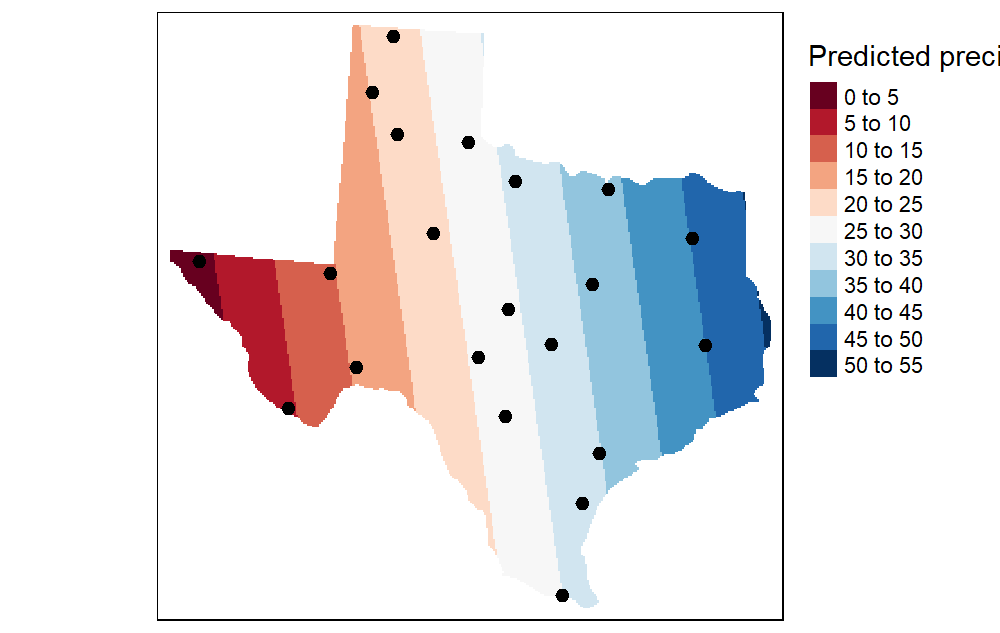
\includegraphics[width=\textwidth]{img/interpolation_fst_order.png}
        \caption{Interpolated values obtained by a $1^{st}$ order trend surface. The model is too rigid.}
        \label{fig:interpolation_fst_order}
    \end{minipage}
    \hfill
    \begin{minipage}{0.49\textwidth}
        \centering
        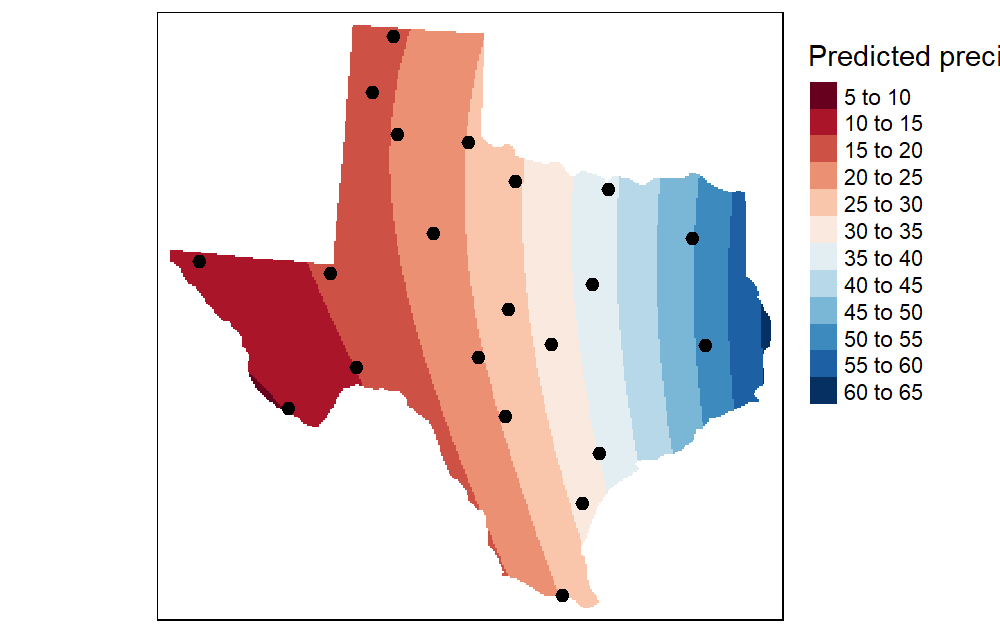
\includegraphics[width=\textwidth]{img/interpolation_snd_order.png}
        \caption{Interpolated values obtained by a $2^{nd}$ order trend surface. The model is better than before, but still not a good fit.}
        \label{fig:interpolation_snd_order}
    \end{minipage}
\end{figure}

\subsubsection{Kriging}

Kriging differs from other methods in that it can assess the quality of prediction with estimated prediction errors. It assumes that the spatial variation of an attribute is neither random nor deterministic; instead, it is a combination of some spatially correlated component, a ``drift'' (assumed for now to be null), and a random error term.

The first step is \textbf{de-trending the data}, so that mean and variance of the data are constant across the whole study area. This can be done by using any trend model and subtracting the predictions from the data. From this point on, the method will focus on residuals, i.e., the remaining variability in te data that is not explained by the global trend. The second step is \textbf{constructing a (semi)variogram}. For each pair of points $i$ and $j$, their semivariance is calculated as:
\begin{equation*}
    \gamma = \frac{(Z_i - Z_j)^2}{2}
\end{equation*}
The variogram is obtained as the plot of all the semivariances, using the $x$ axis to represent distances, and the $y$ axis to represent the semivariances. Usually, it is simplified by binning over the distance values and averaging the semivariances within each bin, obtaining a \textbf{sample experimental variogram}. The third step is to fit an \textbf{experimental variogram model} to find the parameters that best describe the spatial variance; there are many model variants, with the main ones being the Gaussian, linear, and spherical ones. Finally, \textbf{interpolation} can be performed. The general equation for estimating the residual at a point $j$ is:
\begin{equation*}
    z_j = \sum_{i=1}^s z_i W_i
\end{equation*}
where $s$ is the number of sample points used in the estimation, and $W_i$ is the weight assigned to point $i$. These weights are derived by solving a set of simultaneous equations.
\begin{figure}[!ht]
    \centering
    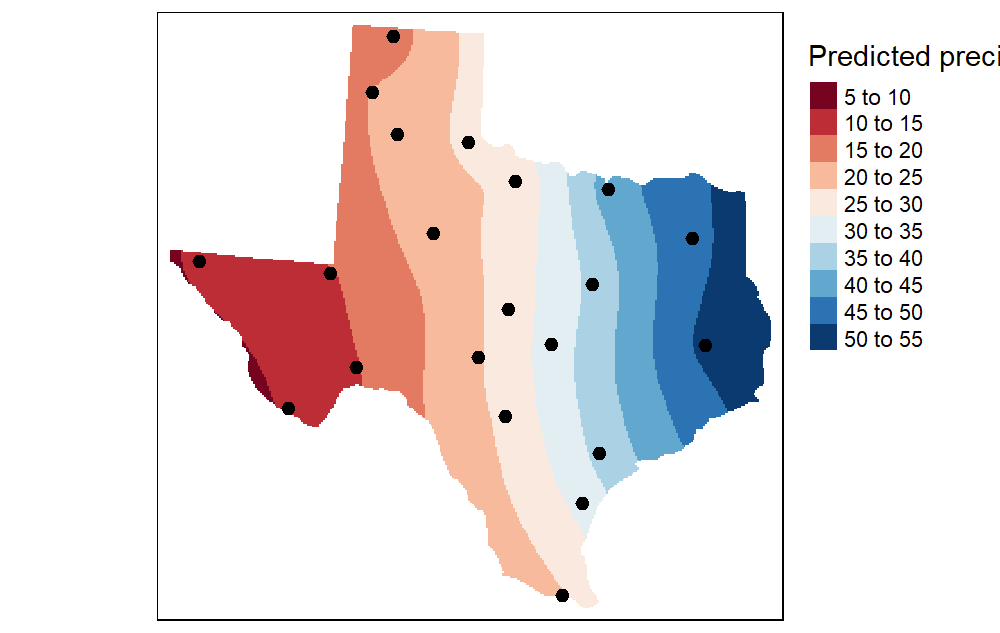
\includegraphics[width=0.5\textwidth]{img/interpolation_kriging.png}
    \caption{Interpolated values obtained by kriging.}
    \label{fig:interpolation_kriging}
\end{figure}

\subsection{Spatial Regression}

Regression has the goal of modeling the relationship between a target variable and a (set of) independent variable(s). The difference with interpolation is that in the latter, only the target variable data and the spatial coordinates are used, while in regression there is information about other non-spatial attributes to make predictions.

Spatial regression extends the typical regression method to include information about a point's neighborhood:
\begin{equation*}
    (P_i) = \underbrace{\alpha + \beta X_i + \epsilon_i}_{\parbox{7.5em}{\scriptsize\centering Standard regression model}} + \underbrace{\delta \sum_j w_{ij} X_j}_{\parbox{7.5em}{\scriptsize\centering Summary information about neighbors}}
\end{equation*}

\section{Co-location Pattern Mining}

Co-location pattern mining is the process of finding subsets of spatial features whose instances are frequently located together in space. It is similar to traditional frequent itemset mining, although defining ``transactions'' is not as immediate, since there is no explicit way to isolate instances into groups.

Given:
\begin{itemize}
    \item A set of features $F = \{f_1, \dots, f_m\}$;
    \item A set of instances $O = \{o_1, \dots, o_n\}$;
    \item A neighbor relation $R$ between pairs of instances, s.t. $R(o_1, o_2) \iff d(o_1, o_2) < \textit{thresh.}$; 
\end{itemize}
a \textbf{co-location pattern} $CL = \{f_1, \dots, f_k\} \subseteq F$ is a subset of features, and an \textbf{instance of a pattern} $I = \{o_1, \dots, o_k\} \subseteq O$ is a subset of objects s.t.:
\begin{itemize}
    \item For each $f \in F$, there is exactly one object $o \in O$ of type $f$, anc vice versa;
    \item $I$ forms a clique w.r.t. $R$ (i.e., all pairs of objects are connected to each other).
\end{itemize}
A co-location pattern that contains $k$ spatial features is called size-$k$ co-location pattern.

To measure the prevalence of a given pattern, we use two measures; the \textbf{participation ratio} (of a feature within a pattern):
\begin{equation*}
    PR(CL, f_i) = \frac{\#|\pi_{f_i} (\textit{instances(CL)})|}{\#|\textit{instances(CL)}|}
\end{equation*}
and the \textbf{participation index} (of the entire pattern):
\begin{equation*}
    PI(CL) = \min_{i=1}^k PR(CL, f_i)
\end{equation*}
A co-location pattern is called \textbf{prevalent} if its partecipation index is greater or equal than a given threshold \textit{minprev}. The participation index is anti-monotone, which means that the participation index of a co-location pattern is always lower or equal to that of its sub-patterns.

\section{Trend Detection}

Spatial trend analysis is the process of finding patterns of change of non-spatial attributes in the neighborhood of some object in the study area. It is analogous to trend analysis in time series, but applied to spatial data, where the linear direction of time is replaced by the many possible paths that can be formed in space. The most notable paths of interest usually start from a common location (e.g., a city center), have meaningful shape, and show a statistically significant trend.

Let $g$ be the neighborhood graph that represents all the neighborhood relationships among objects in the study area. Let $o$ be one such object, which is considered the starting point of paths. Let $a$ be a subset of all non-spatial attributes, in which paths must be found in. Let $t$ be a type of function (e.g., linear, exponential) used for regression. Then, the goal of spatial trend detection is to discover the set of all neighborhood paths in $g$, starting from $o$, having a trend of type $t$ in attributes $a$, with a correlation greater or equal to a given threshold \textit{minconf}.

To isolate these relevant paths, special filters are used to select subsets of all paths. There are many ways to define such filters; some examples are reported in Fig \ref{fig:trend_filters}.
\begin{figure}
    \centering
    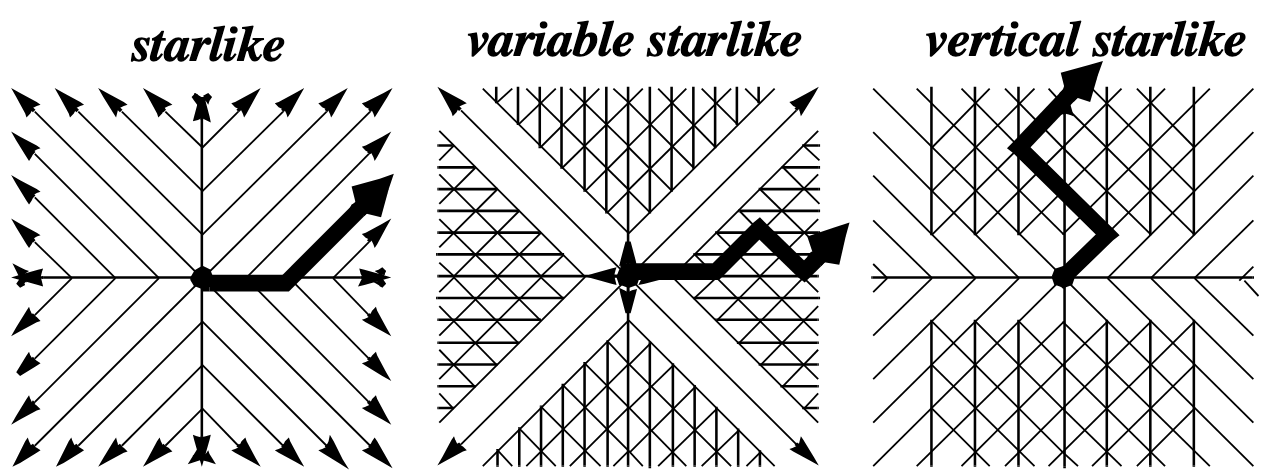
\includegraphics[width=0.75\textwidth]{img/trend_filters.png}
    \caption{Examples of possible filters. The \textit{stralike} filter allows paths that deviate in a specific diagonal direction; the \textit{variable starlike} filter allows paths that can deviate diagonally multiple times; the \textit{vertical starlike} filter restricts horizontal deviations in favor of vertical ones.}
    \label{fig:trend_filters}
\end{figure}